\documentclass[a4paper,12pt]{report}
\usepackage[latin1]{inputenc}
\usepackage[english]{babel}
\usepackage[pdftex]{graphicx} 
\usepackage{sidecap}
\usepackage{pdfpages}
\usepackage{fancyvrb}
\usepackage{floatrow}
\usepackage[section]{placeins}

\bibliographystyle{unsrt}
\begin{document}

\begin{titlepage}
\begin{center}

\includegraphics[width=5cm]{EURECOM_logo_quadri}
\\[3cm]
\textbf{\Huge{Building NERD dashboard}}
\\[2cm]
\textbf{\textsc{\LARGE{Semester Project Report}}}
\\[0.5cm]
\LARGE{Chillari Paolo}
\\
\large{Fall 2011}
\\[8cm]
\columnsep3cm
\begin{tabular}{p{8cm} p{8.5cm}}
\small{\textbf{Supervisors:}\newline
Rapha\"el Troncy\newline
Giuseppe Rizzo} 
&\small{\textbf{EURECOM\newline Multimedia Department}}
\end{tabular}
\end{center}
\end{titlepage}

 \tableofcontents

\chapter{Introduction}
Dashboards have become the de facto face of performance management applications and are increasingly used in business intelligence (BI). The world of web is becoming itself the world of big data, but frequently it's hard to give meaning and extract useful information from this huge amount of bytes. Moreover how this informations are presented to the administrator is critically important and make data understandable to human eyes.

There are zettabytes of data in the world today, and companies, assotiacions, research labs are drowning in information. Dashboards place the data the this entities need in a visual, easy-to-understand format. The ability to see the data that you need, when you need it, gives you the ability to quickly understand the current situation at any given point in time. Rather than digging through databases, logs files, spreadsheet you can consult your dashboard for a quick insight.

A dashboard democratizes access to big data, so that anyone  can have the right information at their fingertips.

Dashboard has become integral and substantive part of web application panorama giving privates, companies, IT service providers, etc the ability to handle their business efficiently. Dashboard, as a matter of fact, could achieve different goals, from strategic to analytical or operational requirements.
The main focus of this project is on Administration Dashboards, where admins can have a full overview of what is happening on their platform. The dashboard summarizes in one single location all the informations that an administrator need: from user's informations to how many visits, page-views and other detailed information about the platform. In some cases, like for the Nerd Application, should provide a common interface for interacting with data stored by your site.

\chapter{Similar projects}

The web panorama is full of great example of dashboard and how they became the pivot of huge businesses.
We analyze to great examples Google Analytics and 3scale.
\section{Google Analytics}
Google analytics is ....
\section{3scale}
3scale is a management solutions for developers, and companies to securely distribute, control, manage, operate and monetize their API. His API management platform is Plug and Play, configurable, flexible and scalable and brings API providers an unparalleled level of ownership, control and configuration to ensure QoS, SLA and a great user experience.
3Scale exposes a Dashboard to monitor the API usage, in order to give the developer a full overview and control of the usage of his APIs.
3scale shares with NERD some key point and therefore it  represents a good case of study.

The main features:
\begin{itemize}
\item[Usage] \hfill \\
 3Scale exposes a time-line chart to show the total usage of the apis. The timeline is navigable in time and the dashboard admin could filter data by  metrics or API methods.

\item[Top Applications] \hfill \\
As for the usage, we have a another time-line chart. One of the cool features of 3Scale is that the developers has a full overview of the usage of his APIs for every application that is using it. As before we can choose metrics and methods.
Hour of day and day of week

\item[Daily and weekly usage] \hfill \\
 3Scale dashboard also allow to aggregate by the hours of the day and the days of the week. In order to take under control the load in different time of the day or different days of the week


\item[Other features] \hfill \\
As the others main dashboard services 3Scale allow to define alerts, in order to give the developer updates about data that he cares most.
\end{itemize}

\chapter{Dashboard Design Study}
\section{Framing the Dashboard - Structure}
This section offers ideas about the big-picture elements of the building blocks that has to be use to construct a dashboard. The building blocks can be broken into four categories.
\subsection{Form}
It's important to select the form that fits the needs of the situation.
The goal is to show critical information in a way understandable and in order to be available when the audience needs it.
\begin{itemize}
\item[Timeliness] \hfill \\
Frequency of  data update
According to the most popular dashboard and, first of all, to Google Analytics, data's update follows two main patterns: data  is displayed and updated in response of a request made directly by the administrator on the User Interface 
The second pattern, which is commonly in parallel, is to have a section where  data is displayed in real time.Thus the administrator could see what is happening on the framework in that moment. Concerning Nerd Dashboard the administrator could have, for example, a global overview of the usage of the rest APIs, how much users are currently using it, from where, what are the REST methods and entities accessed.
\item[Aesthetic] \hfill \\
For the Nerd framework this could be not the most urgent and important feature to achieve, but for a personal point of view and according to the JUICE article a good aesthetic reflects the usability and makes the accessibility to  data easiest.
In fact Google Analytics in the last years put a lot of efforts to change and improve the UI and aesthetic of the dashboard.
\item[Mobility] \hfill \\
Since administrators of Nerd has to travel all around the world, the chance to access data on the go is an important feature. Administrators need to have data accessible from everywhere using laptops but also tablets and smartphone in order to obtain a full overview of the dashboard in every moment they need to.
\item[Connectivity] \hfill \\
Depending on the amount of data that has to be accessed and how the administrator has to filter and parametrize data is it possible to follow different patterns. 
In order to achieve the real time features the backend module that handle the dashboard has to talk directly with data-source and the NerdFramework server.
\item[Data detail] \hfill \\
The administrator has to access data in detail, dive into all the information stored on the database. But this data has to be presented in the right way in order to avoid  be a a mess of meaningless numbers.
\item[Data density] \hfill \\
 How much information rich will views of the data be? The best structured way to achieve a balance data density is to reveal information as the administrator expresses interest. In other words, don't bombard the admin with all the information at once using levels of increasing detail from 
\item[Interactivity] \hfill \\ 
The Nerd Admin has to actively interact with the dashboard in order to organize, filter, define metrics on the data he needs. A great dashboard requires to be customizable and, especially for Nerd, the Admin has to fully interact with the data that comes from it.
\item[Collaboration] \hfill \\
There is a team working on the network so it could be the need to cooperate on the framework. But I think that for Nerd the dashboard could not be the right tool to achieve this collaboration, there are betters tools that are born to handle collaboration in the field of Computer Science Development and Research. 
I see this tool more for a business or strictly administration dashboards.
\end{itemize}
\subsection{Structure}
\emph{``Dashboard content must be organized in a way that reflects the nature of the information and that supports efficient and meaningful monitoring. Information cannot be placed just anywhere on the dashboard.''}\newline
\emph{``Important items should often appear larger, thus more visually prominent, than less important items''}

\begin{itemize}
    \item \textbf{Flow}\newline
    A flow-based structure emphasizes a sequence of events or actions across time
    \item \textbf{Relationship}\newline
    The structure of a dashboard can also emphasize the relationships between entities or measures. These relationships or connections may be mathematical, geographical or functional.
    \item \textbf{Grouping}\newline
    The structure of last resort is to group related information into categories or a hierarchy. The structure of last resort is to group related information into categories or a hierarchy
\end{itemize}
\subsection{Design Principles}
Few core design goals that as to be reminded as you get closet to start sketching your application: is quite difficult to straightly follow simultaneously all these key design principle, instead it's better to pick one or two with higher priority to help stay focused.
\begin{itemize}
    \item \textbf{Compactness/Modularity}\newline
    Dashboard could become large and unwieldy, especially when it tries to give a comprehensive view of huge business that could be, in their fullness, various and heterogeneous. Compactness is the property that a design can fit inside a human being's head
    A dashboard can be broken into bite-sized pieces, each built around a key question in order to be organized and give to the administration a more organized and ordained view.
    \item \textbf{Gradual reveal}\newline
    Reveal information as the dashboard user expresses interest. Don't bombard the administrator with all the information at once (use levels of increasing details)
    \item \textbf{Customizable}\newline   
    Allow users to customize the dashboard (defining the scope). 
    Does the dashboard let the admin save a view of the data that they have configured? \newline
    Does it offers easy ways to tag or highlight things that are important to them?
    \item \textbf{Explanation before information}\newline
    Dashboards need to give the context and explanation to understand new and unfamiliar events.Letting the data speak for itself can be a recipe for misinterpretation and confusion.
\end{itemize}

\subsection{Functionalities}
\begin{itemize}
\item \textbf{Filters}\newline
Allow users to define the scope of the data in the dashboard to reflect their needs. Filters can either be global (refining scope for the entire dashboard) or local(refining scope for a specific chart or metric or view).

\item \textbf{Comparison}\newline
Ability to see two or more subsets of the data side-by-side. A line chart, for example, may let the the Admin view two geographic regions as separate lines or in the same chart lines of different colors for the same source of data with different filters applied

\item \textbf{Alerts}\newline
Highlight information based on pre-defined criteria. Alerts may be activated when a metric goes outside of a particular threshold.  The administrator could define alerts for instance when a threshold for a first class object is reached, based on some predefined filters and more in general on whatever could be a matter of statistics both in absolute and relative value.

\item \textbf{Export / print}\newline
The  admin should have the ability to export data out of the dashboard in different formats. In details, should be possible to not only export all the data available but the exported data should reflect filters, metrics, parameters that the administrator could defined: for instance every personalized widget should be exportable as a chart or as a table of data.
\end{itemize}

\section{Information Design}
In this last part we provide practical tips for putting information on the page in a way that communicates effectively to our audience. How data is presented is a primary goal and it strongly affects the final result. Best practices for designing a clear, aesthetically-pleasing page are key factors.\newline
A clear and simple interface is the primary goal and deals with limiting visual clutter to allow the user to easily navigate and understand the content on th page.

\begin{itemize}
\item \textbf{Organizing the page: } information could not be just arranged on the page without order, semantics and taking into account where people looks first, where information should be to capture user's attention.
Moreover a \"grid system\" approach brings order and coherence into the page. Finally white space can be used to delineate sections or help users see groupings of content in a dashboard. Using white space may means sacrificing one extra chart or metric, but it can make a huge difference in user comprehension.

\item \textbf{Colors:}
Appropriate use of color requires restraint. In our dashboard designs, we typically start by using only grey and then add colors where it conveys useful information.
Colors bring meaning: they can draw your eye to what is important and tie together similar things.but there is a critical mid-point and categorical when data falls into distinct groups.

\item \textbf{Typography: }it includes everything from choosing a typeface to picking the right point size, kerning, tracking and leading.
Simple font framework:
\begin{itemize}                                    
\item Body text is clean, readable content
\item Headers separate and name major sections of the work                                                       
\item Notes describe additional things the reader should be aware of. These should fade into the background unless we call attention to them.
\item Emphasis text is what we want our reader to pay particular attention to.   
\end{itemize}
\end{itemize}

(i.e. font) to picking the right point size, kerning, tracking, and leading. In the meantime,
\chapter{Designing NERD dashboard}

\section{Sketching}
Sketches are a crucial phase of our project and represents the start point of the dashboard design. The Dashboard Design Study described in Chapter 2 is the guideline and we tries to follow the best-practices.
Moreover, what strongly characterize our sketches is the purpose of build a fully responsive web app: 
\begin{quote} 
    Responsive Web Design (RWD) is a web design approach aimed at crafting sites to provide an optimal viewing experience-easy reading and navigation with a minimum of resizing, panning, and scrolling-across a wide range of devices (from desktop computer monitors to mobile phones).
\end{quote}
The world is changing fast and day by day, the number of devices, platforms, and browsers that need to work on the web grows dramatically. Responsive web design represents a fundamental shift in how we'll build websites for the decade to come.
Smartphones, tablets, Internet connected Tvs are becoming more and more popular bringing the problem of fragmentation to be put in the foreground.
In our project we handle this problem, starting from this first part: we decided to use an off canvas pattern for multi-device: this layout takes advantage of space off the screen to keep content or navigation hidden until either a larger screen size allows it to be visible or a user takes action to expose it.
\\[0.2cm]
\begin{figure}[htbp]
  \caption{Facebook example of Off Canvas Pattern .}
  \centering
    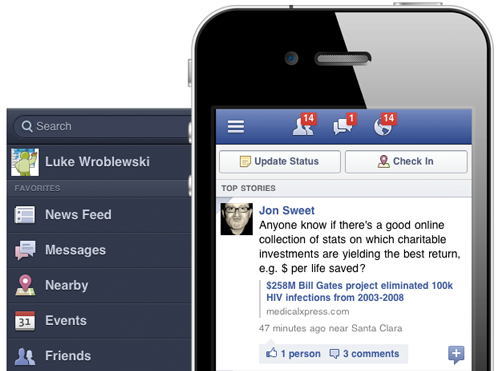
\includegraphics[width=0.7\textwidth]{pics/UISketches/offCanvas}
\end{figure}

The Off Canvas pattern is a interesting one because it doesn't force people to scroll long pages of content and navigation on small screens.1 Instead sections can be separated, labeled, and accessed when needed.


\subsection {Mobile UI}
It's becoming shared thinking that, to create a compelling and responsive website, it helps to focus first on smartphone users: start your design for small touchscreens and scale up from there. This can help ensure that a web application satisfies users on any device and loads quickly on any type of Internet connections.

% \begin{figure}
%   \centering
% \includegraphics[height=0.7\textwidth]%
%     {pics/UISketches/mobileSk1}% picture filename
%   \caption{ This sketch represents the view of one section of the dashboard, the contents fully occupies the page size, exploiting all the space and thus allowing the user to have charts and informations larger on the page.}
% \end{figure}


\begin{figure}
\floatbox[{\capbeside\thisfloatsetup{capbesideposition={left,top},capbesidewidth=4cm}}]{figure}[\FBwidth]
{\caption{This sketch represents the view of one section of the dashboard. Contents fully occupy the page, exploiting all the space allowing the user to have charts and informations larger and more readable.}\label{fig:test}}
{\includegraphics[width=5cm]{pics/UISketches/mobileSk1}}
\end{figure}



% \begin{figure}
%   \centering
% \includegraphics[height=0.7\textwidth]%
%     {pics/UISketches/mobileSk2}% picture filename
%   \caption{ This sketch represents the step forward the interaction with the icon floated left on the top bar. The menu slides right and the content with him: now the space is optimized for displaying the sidebar and allowing the user to easily interact with the navigation items }
% \end{figure}


\begin{figure}
\floatbox[{\capbeside\thisfloatsetup{capbesideposition={right,top},capbesidewidth=4cm}}]{figure}[\FBwidth]
{\caption{This sketch represents the step forward the interaction with the icon floated left on the top bar. The menu slides right and the content with him: now the space is optimized for displaying the sidebar and allowing the user to easily interact with the navigation items}\label{fig:test}}
{\includegraphics[width=5cm]{pics/UISketches/mobileSk2}}
\end{figure}

\begin{figure}
\floatbox[{\capbeside\thisfloatsetup{capbesideposition={left,top},capbesidewidth=4cm}}]{figure}[\FBwidth]
{\caption{This sketch represents the interface to modify the options for a chart: everything goes on the background and the options panel occupies the majority of the page}\label{fig:test}}
{\includegraphics[width=5cm]{pics/UISketches/mobileSk3}}
\end{figure}
\FloatBarrier

% \begin{figure}
%   \centering
% \includegraphics[height=0.7\textwidth]%
%     {pics/UISketches/mobileSk3}% picture filename
%   \caption{ This sketch represents the interface to modify the options for a chart: every thing goes on the background and the options panel occupies the majority of the page }
% \end{figure}


\subsection{ Tablet and Desktop UI  }

As suggested by the  the Off Canvas Pattern, shifting on larger screens, more and more content is visible. In our case, the sidebar menu is visible and allow a straight forward navigation in each section of the dashboard. However we decided to leave the user the possibility to close the sidebar and shift in \"Full screen mode\" to fully exploit the space provided by his larger screen. Moreover, to improve the users of bigger devices is possible to change layout of the content page to pick the one most suitable for him.
\begin{figure}[h!]
  \caption{Overview}
  \centering
    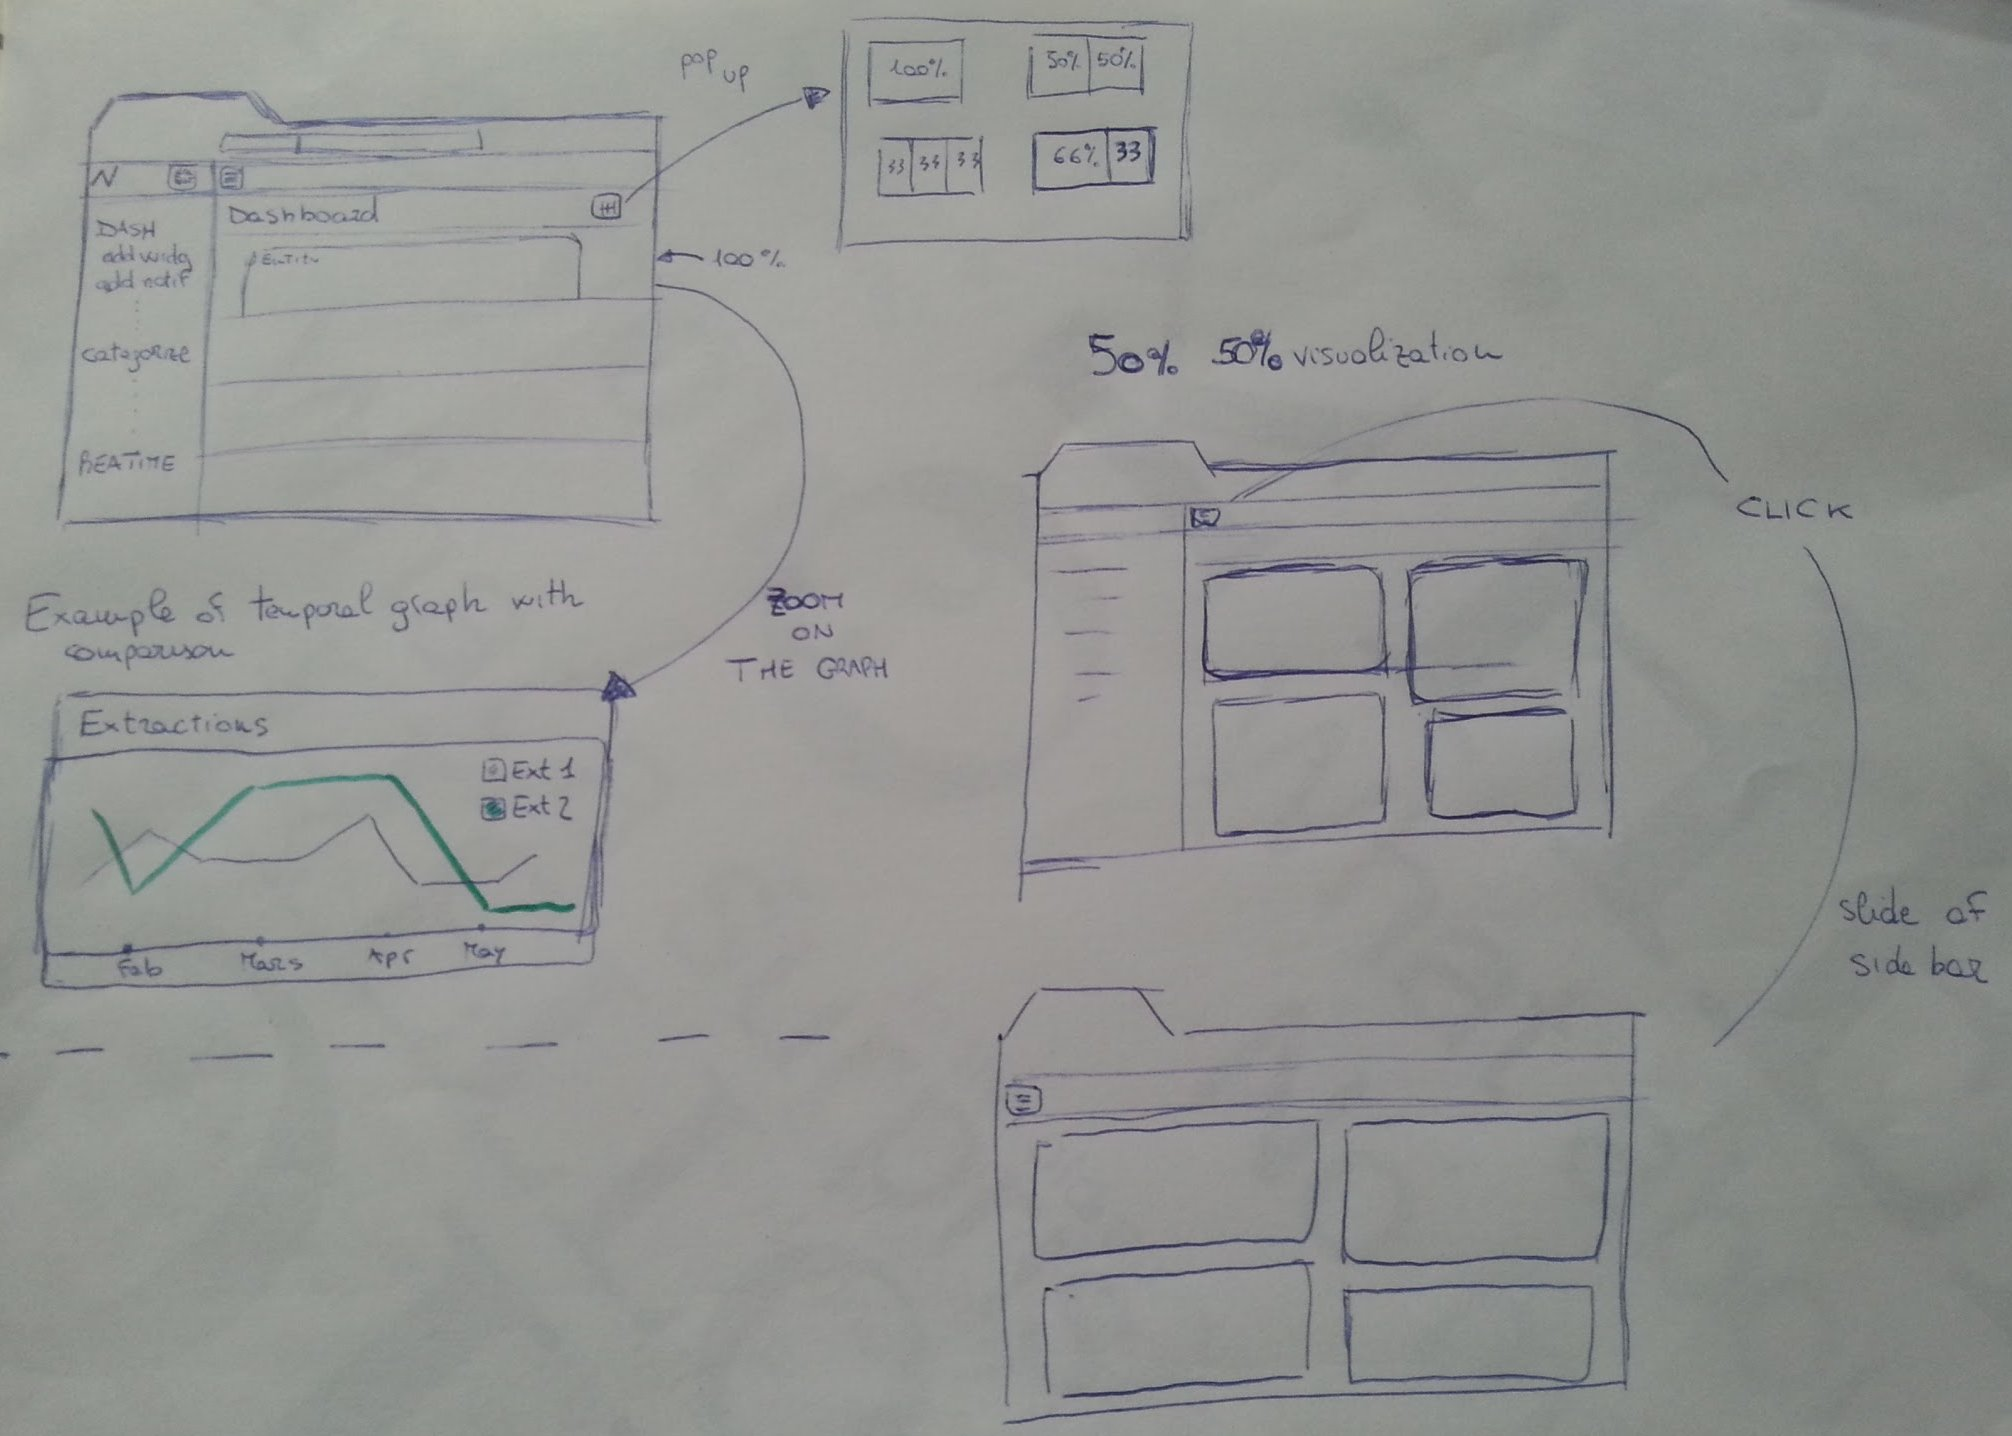
\includegraphics[width=1\textwidth]{pics/UISketches/desk0}
\end{figure}

\begin{figure}
\floatbox[{\capbeside\thisfloatsetup{capbesideposition={left,top},capbesidewidth=4cm}}]{figure}[\FBwidth]
{\caption{This sketch represents the view of one section of the dashboard, the sidebar is visible and allow to directly navigate the dashboard. Timeline, pie, bar charts are the real content of the page}\label{fig:test}}
{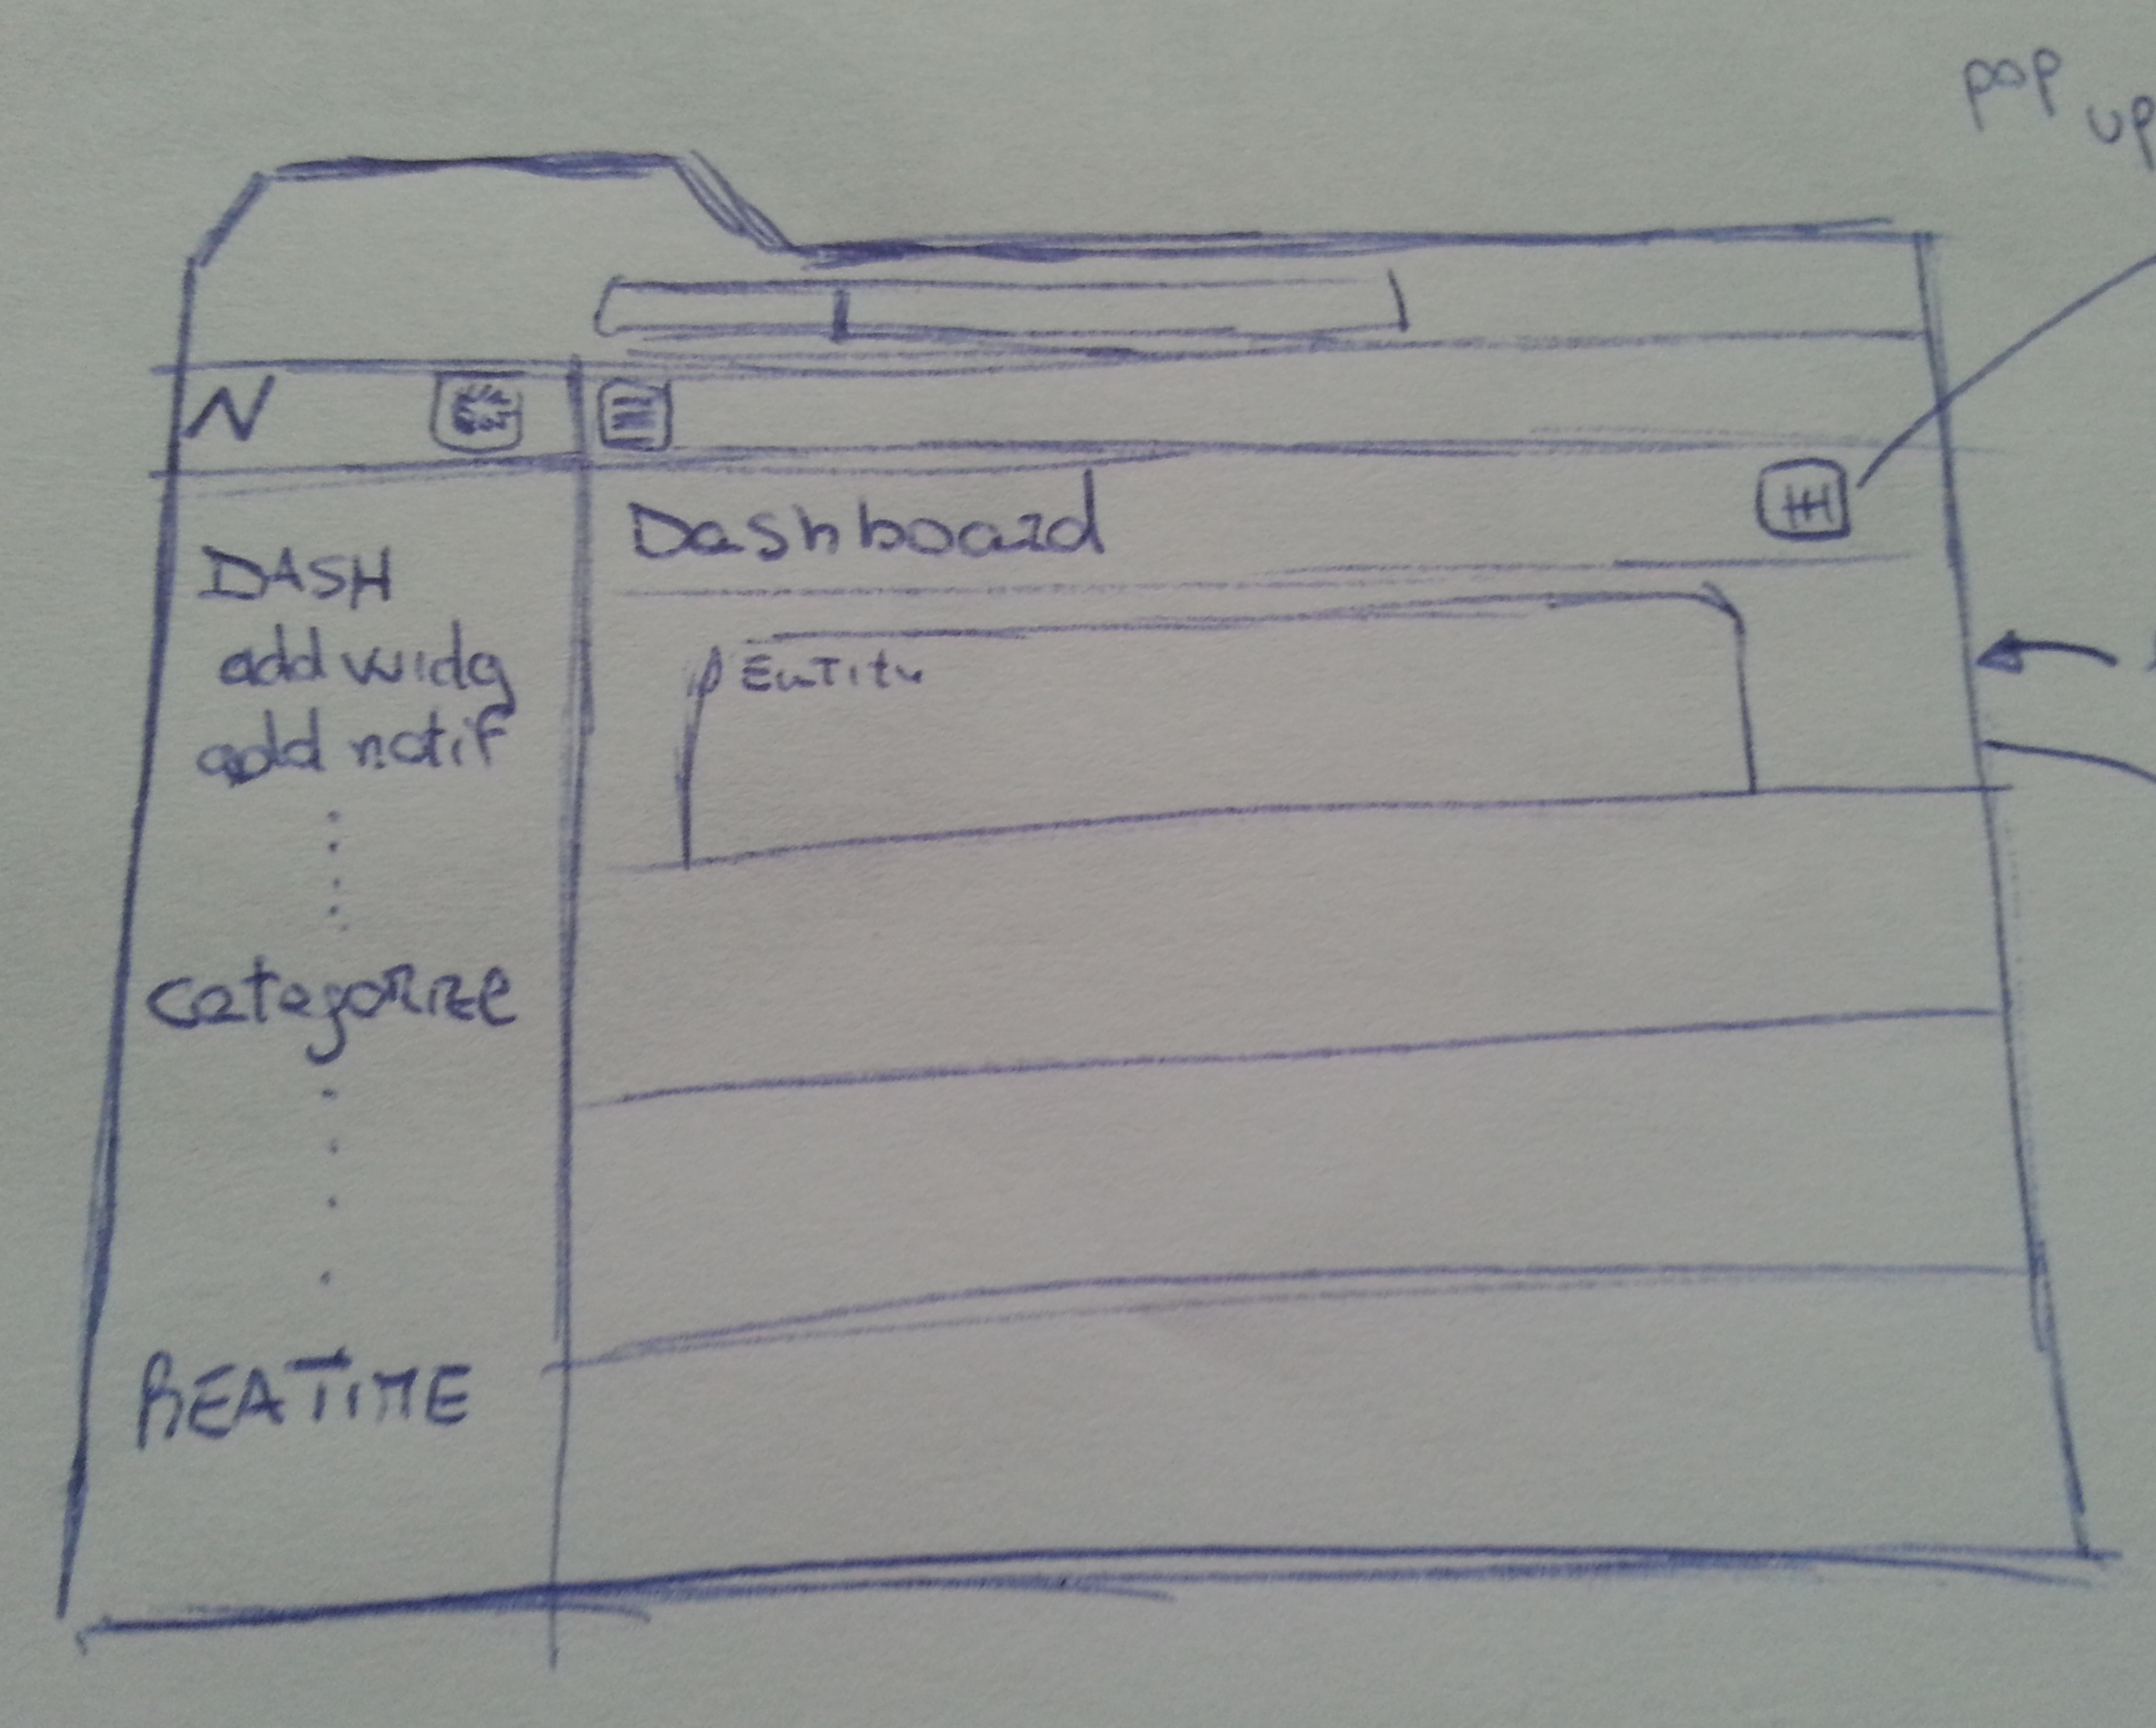
\includegraphics[width=8cm]{pics/UISketches/desk1}}
\end{figure}

\begin{figure}
\floatbox[{\capbeside\thisfloatsetup{capbesideposition={right,top},capbesidewidth=4cm}}]{figure}[\FBwidth]
{\caption{From this panel, directly accessible to each section of the dashboard, the user could choose the most suitable layout, choosing between: 100, 50-50, 33-33-33, 33-66. This different configurations allow to have data differently organized in the page. }\label{fig:test}}
{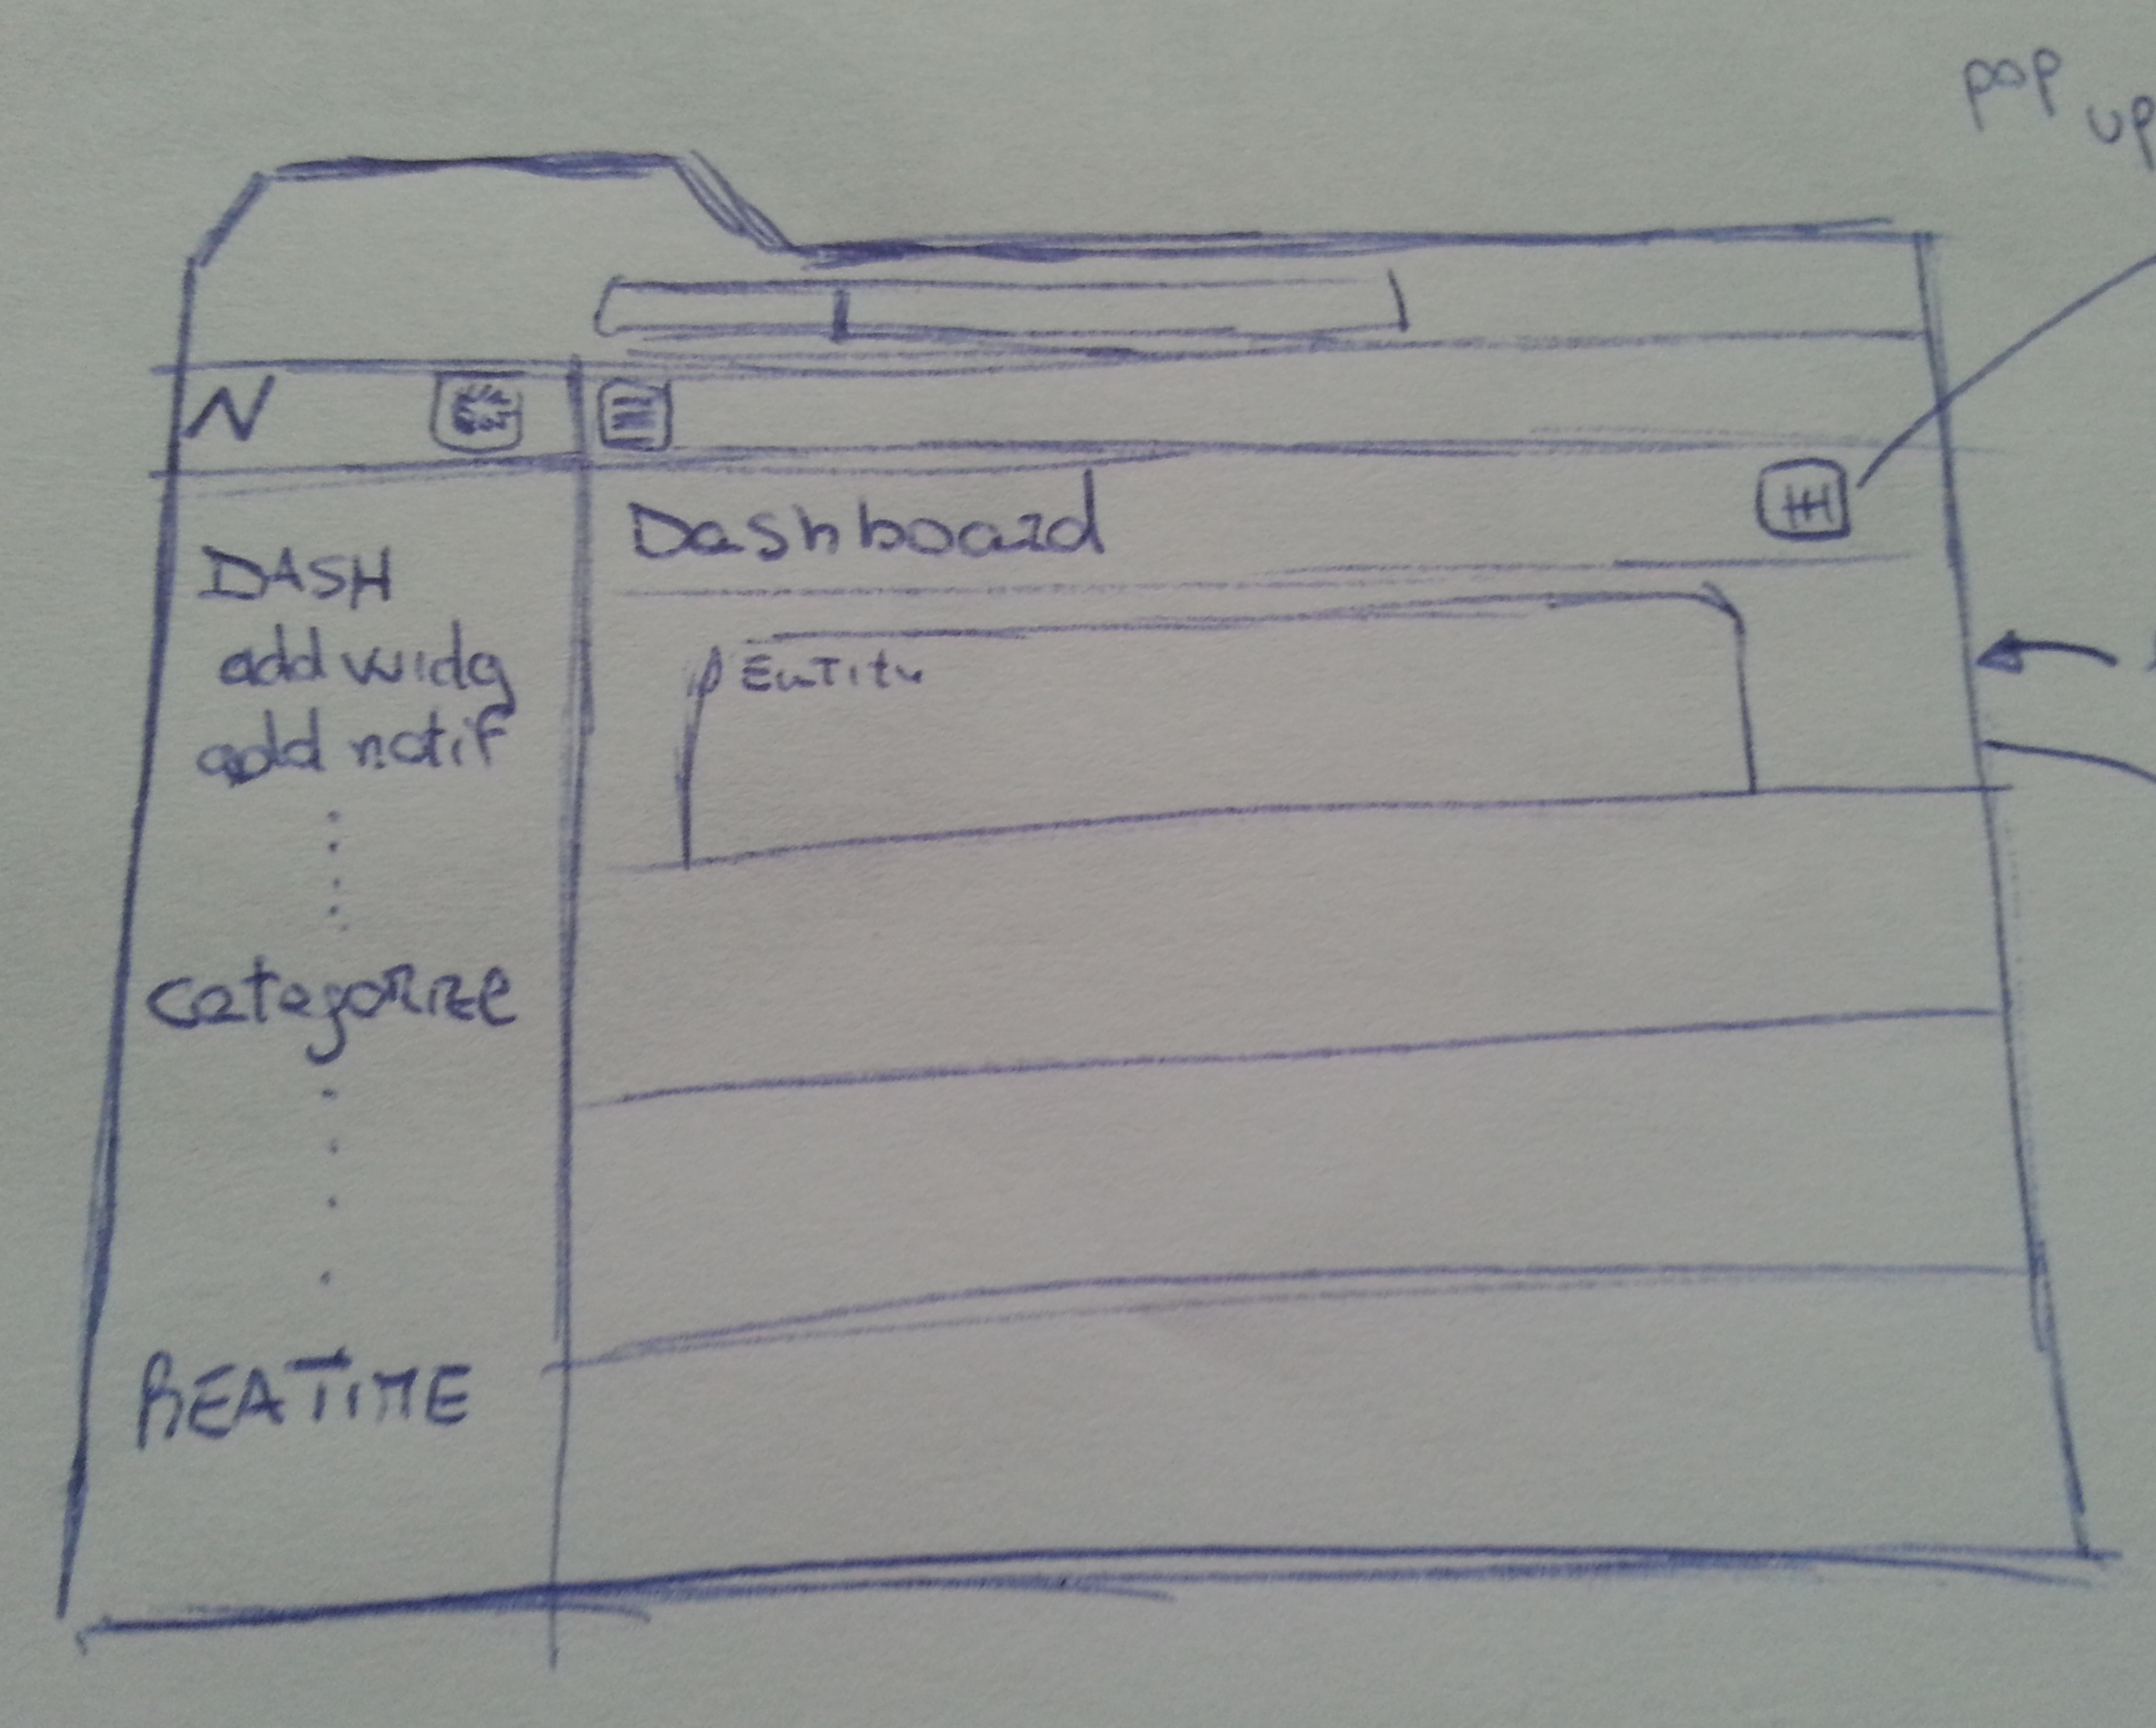
\includegraphics[width=8cm]{pics/UISketches/desk1}}
\end{figure}


\begin{figure}
\floatbox[{\capbeside\thisfloatsetup{capbesideposition={left,top},capbesidewidth=4cm}}]{figure}[\FBwidth]
{\caption{This is an example of 50-50 layout making the data visualization more compact and allowing users to have the focus on more charts than the 100\% one.}\label{fig:test}}
{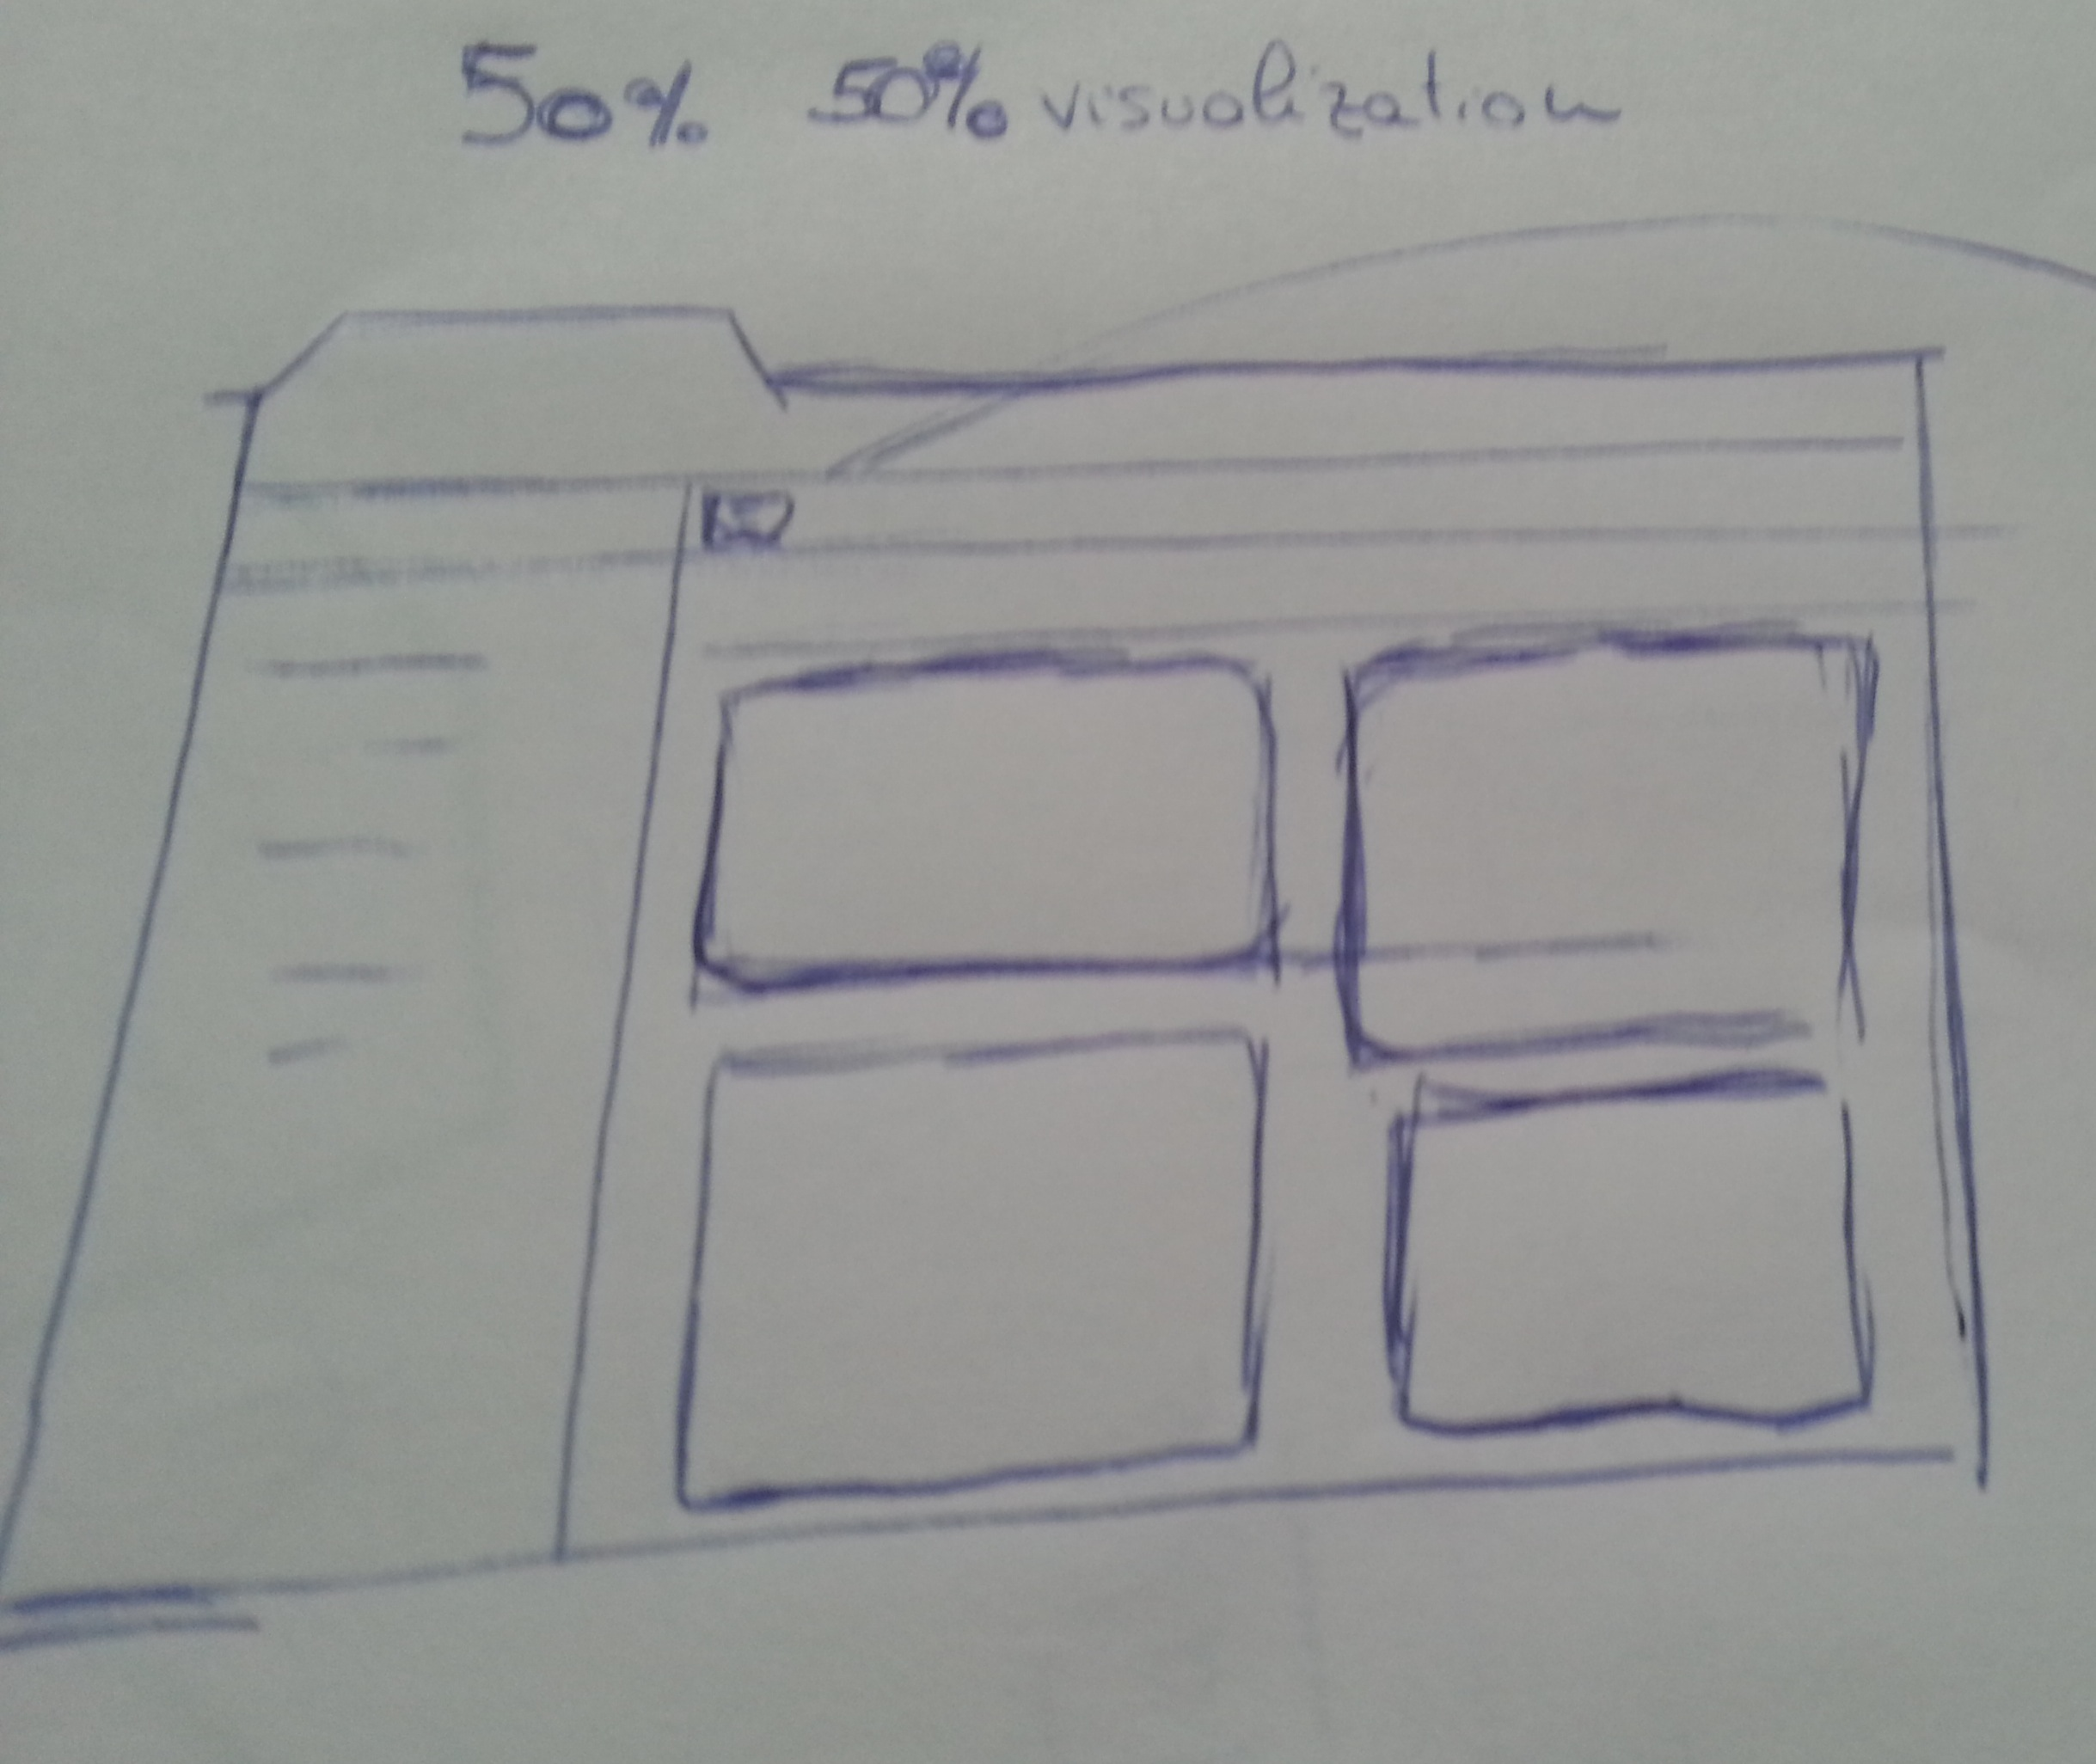
\includegraphics[width=8cm]{pics/UISketches/desk3}}
\end{figure}

\begin{figure}
\floatbox[{\capbeside\thisfloatsetup{capbesideposition={right,top},capbesidewidth=4cm}}]{figure}[\FBwidth]
{\caption{This is an example of 50-50 layout in Full Screen Mode. This visualization allows to fully exploit the size of the screen: the user can focus on data without any distraction}\label{fig:test}}
{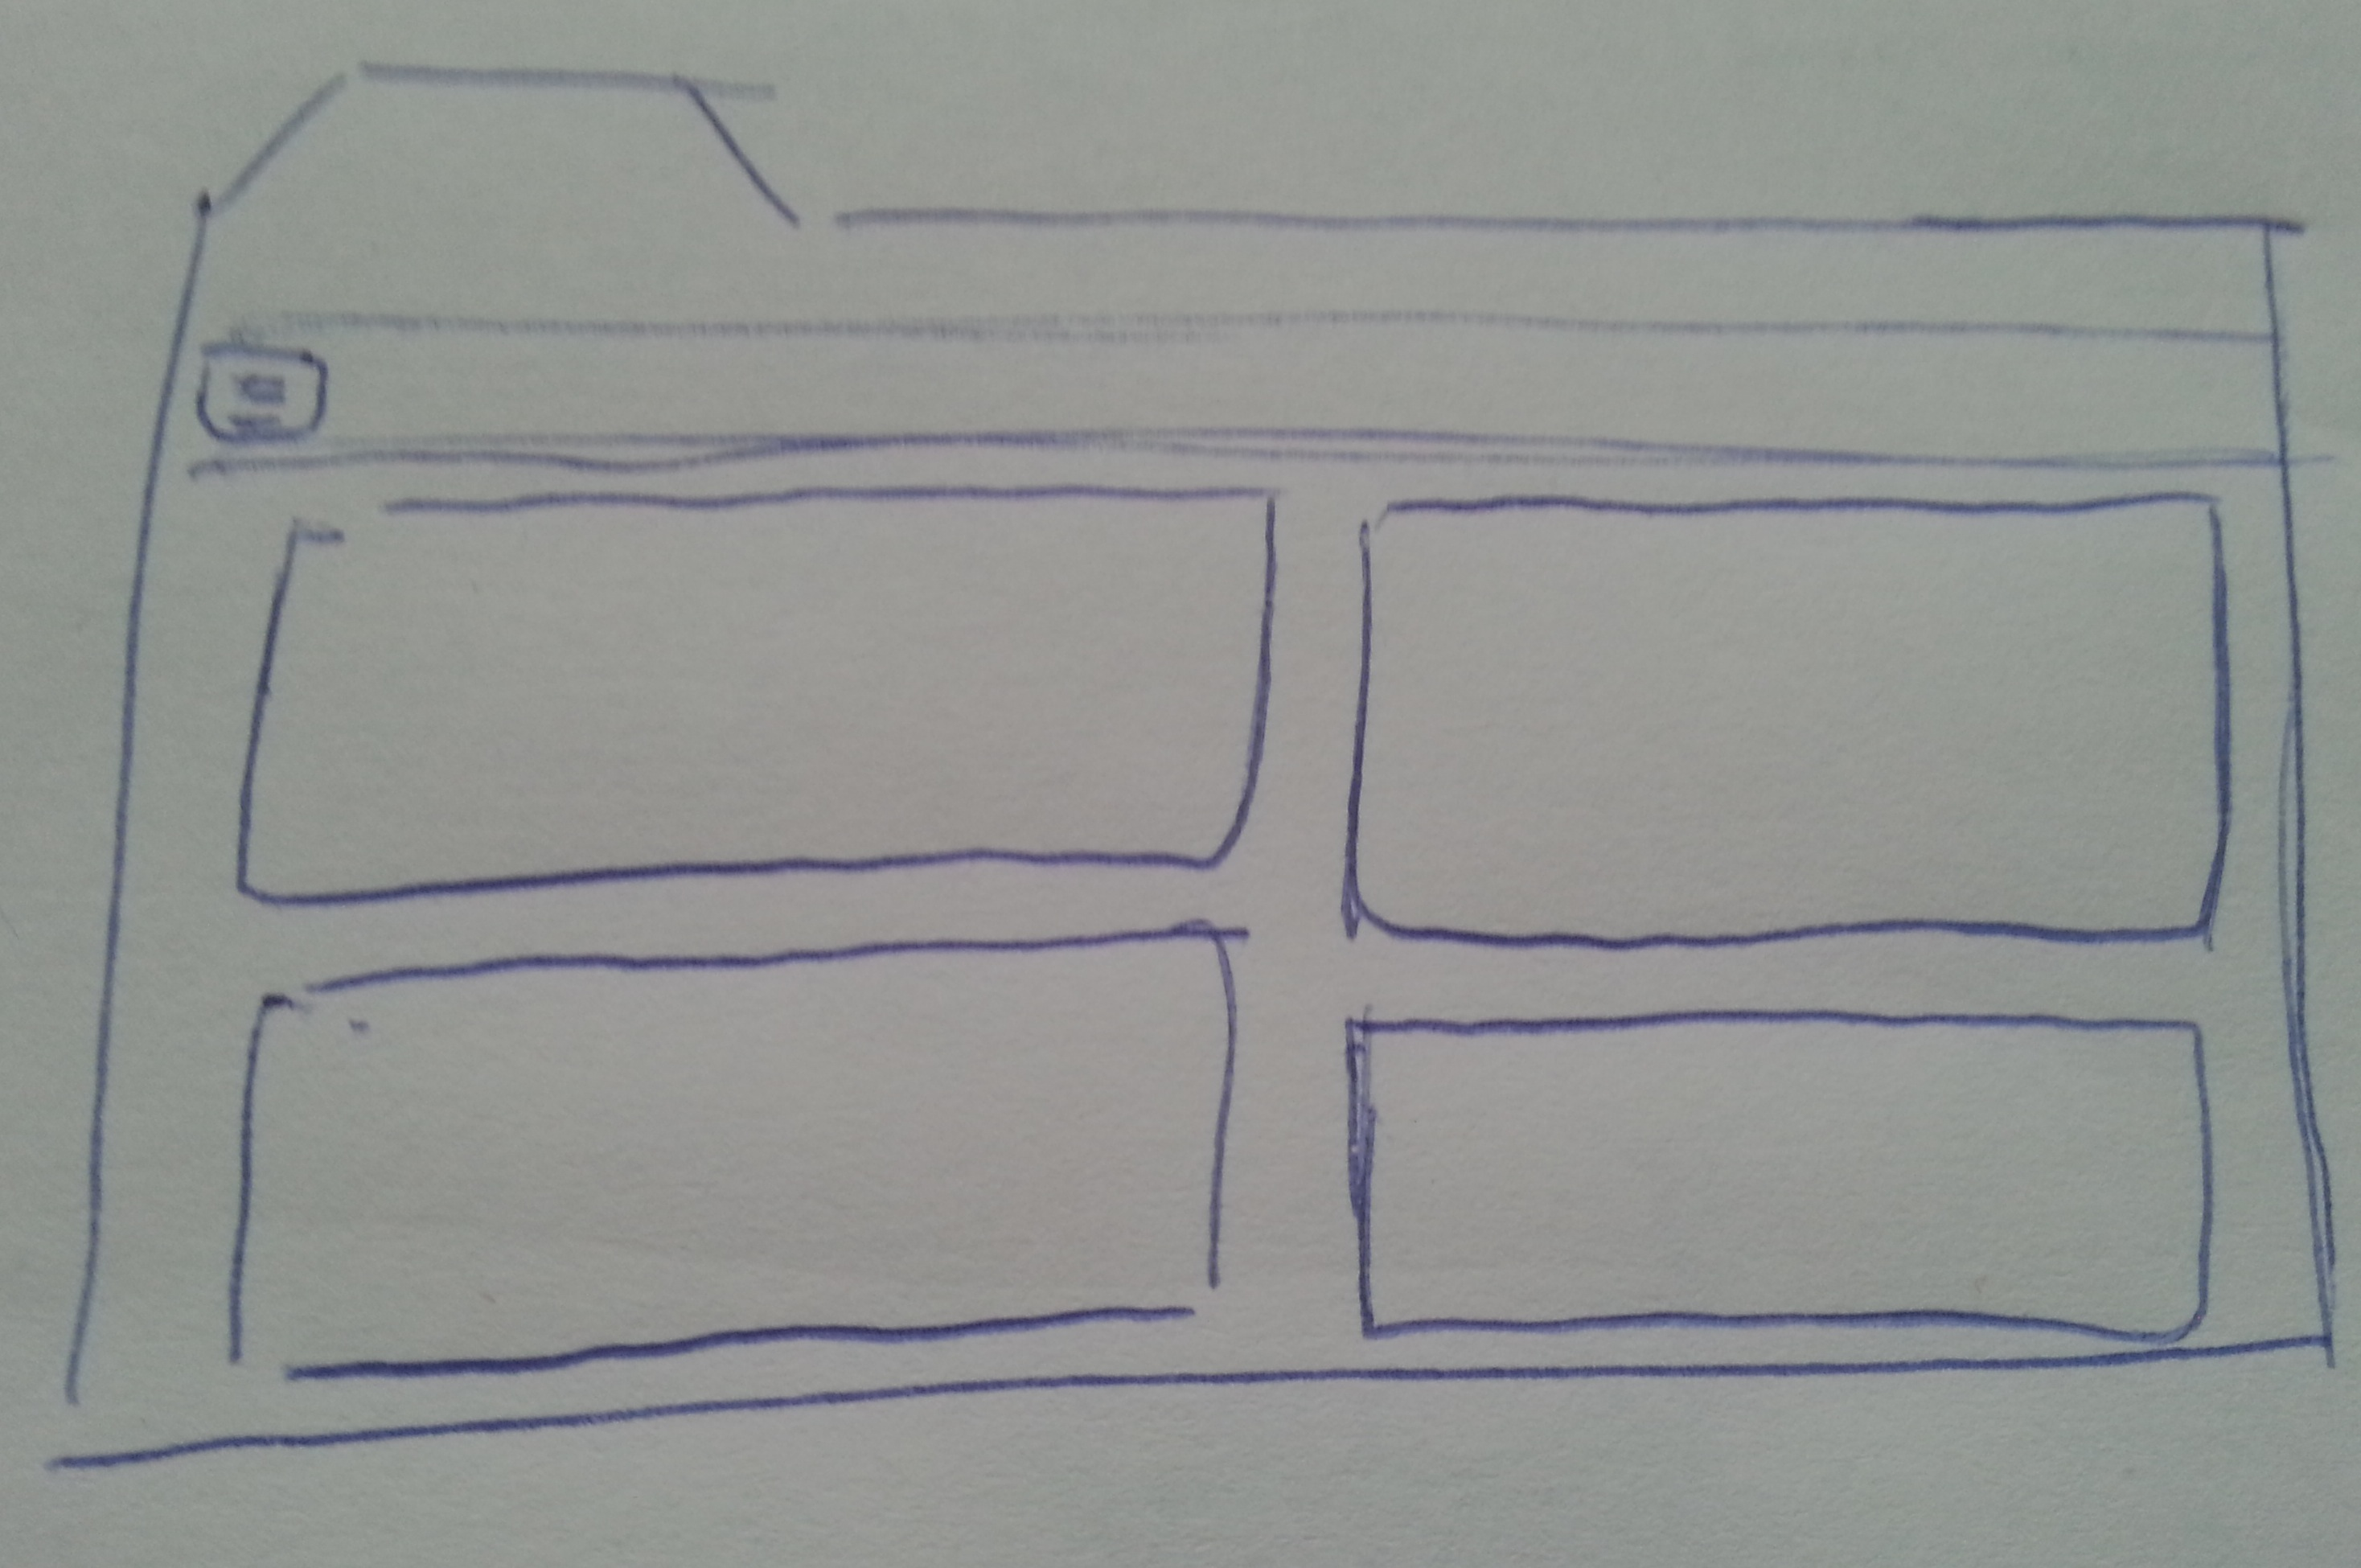
\includegraphics[width=8cm]{pics/UISketches/desk4}}
\end{figure}
\FloatBarrier

\subsection{ Charts }
A dashboard needs to tell a story with data: charts and 
tables are the means to highlight the right information and make them easy to read. It's critically important to choose the right chart for the right data and to design charts visualization following this six guidelines:
\begin{itemize}
\item \textbf{Decrease data-to-ink ratio } 
\item \textbf{Maximize contrast }  Maximize the contrast between your data and the background
\item \textbf{Readable Labels } 
\item \textbf{Avoid smoothing and 3D }  Maximize the contrast between your data and the background
\item \textbf{Sort for comprehension }
\item \textbf{Use color variants }  
\end{itemize}
Starting from this principles and thinking on the type of data to display we came up with the following sketches.

\begin{figure}
\floatbox[{\capbeside\thisfloatsetup{capbesideposition={right,top},capbesidewidth=4cm}}]{figure}[\FBwidth]
{\caption{This is how the graph panel should appear on the page: a top bar with the chart title(and possible icons for interaction), the graph itself and a legend}\label{fig:test}}
{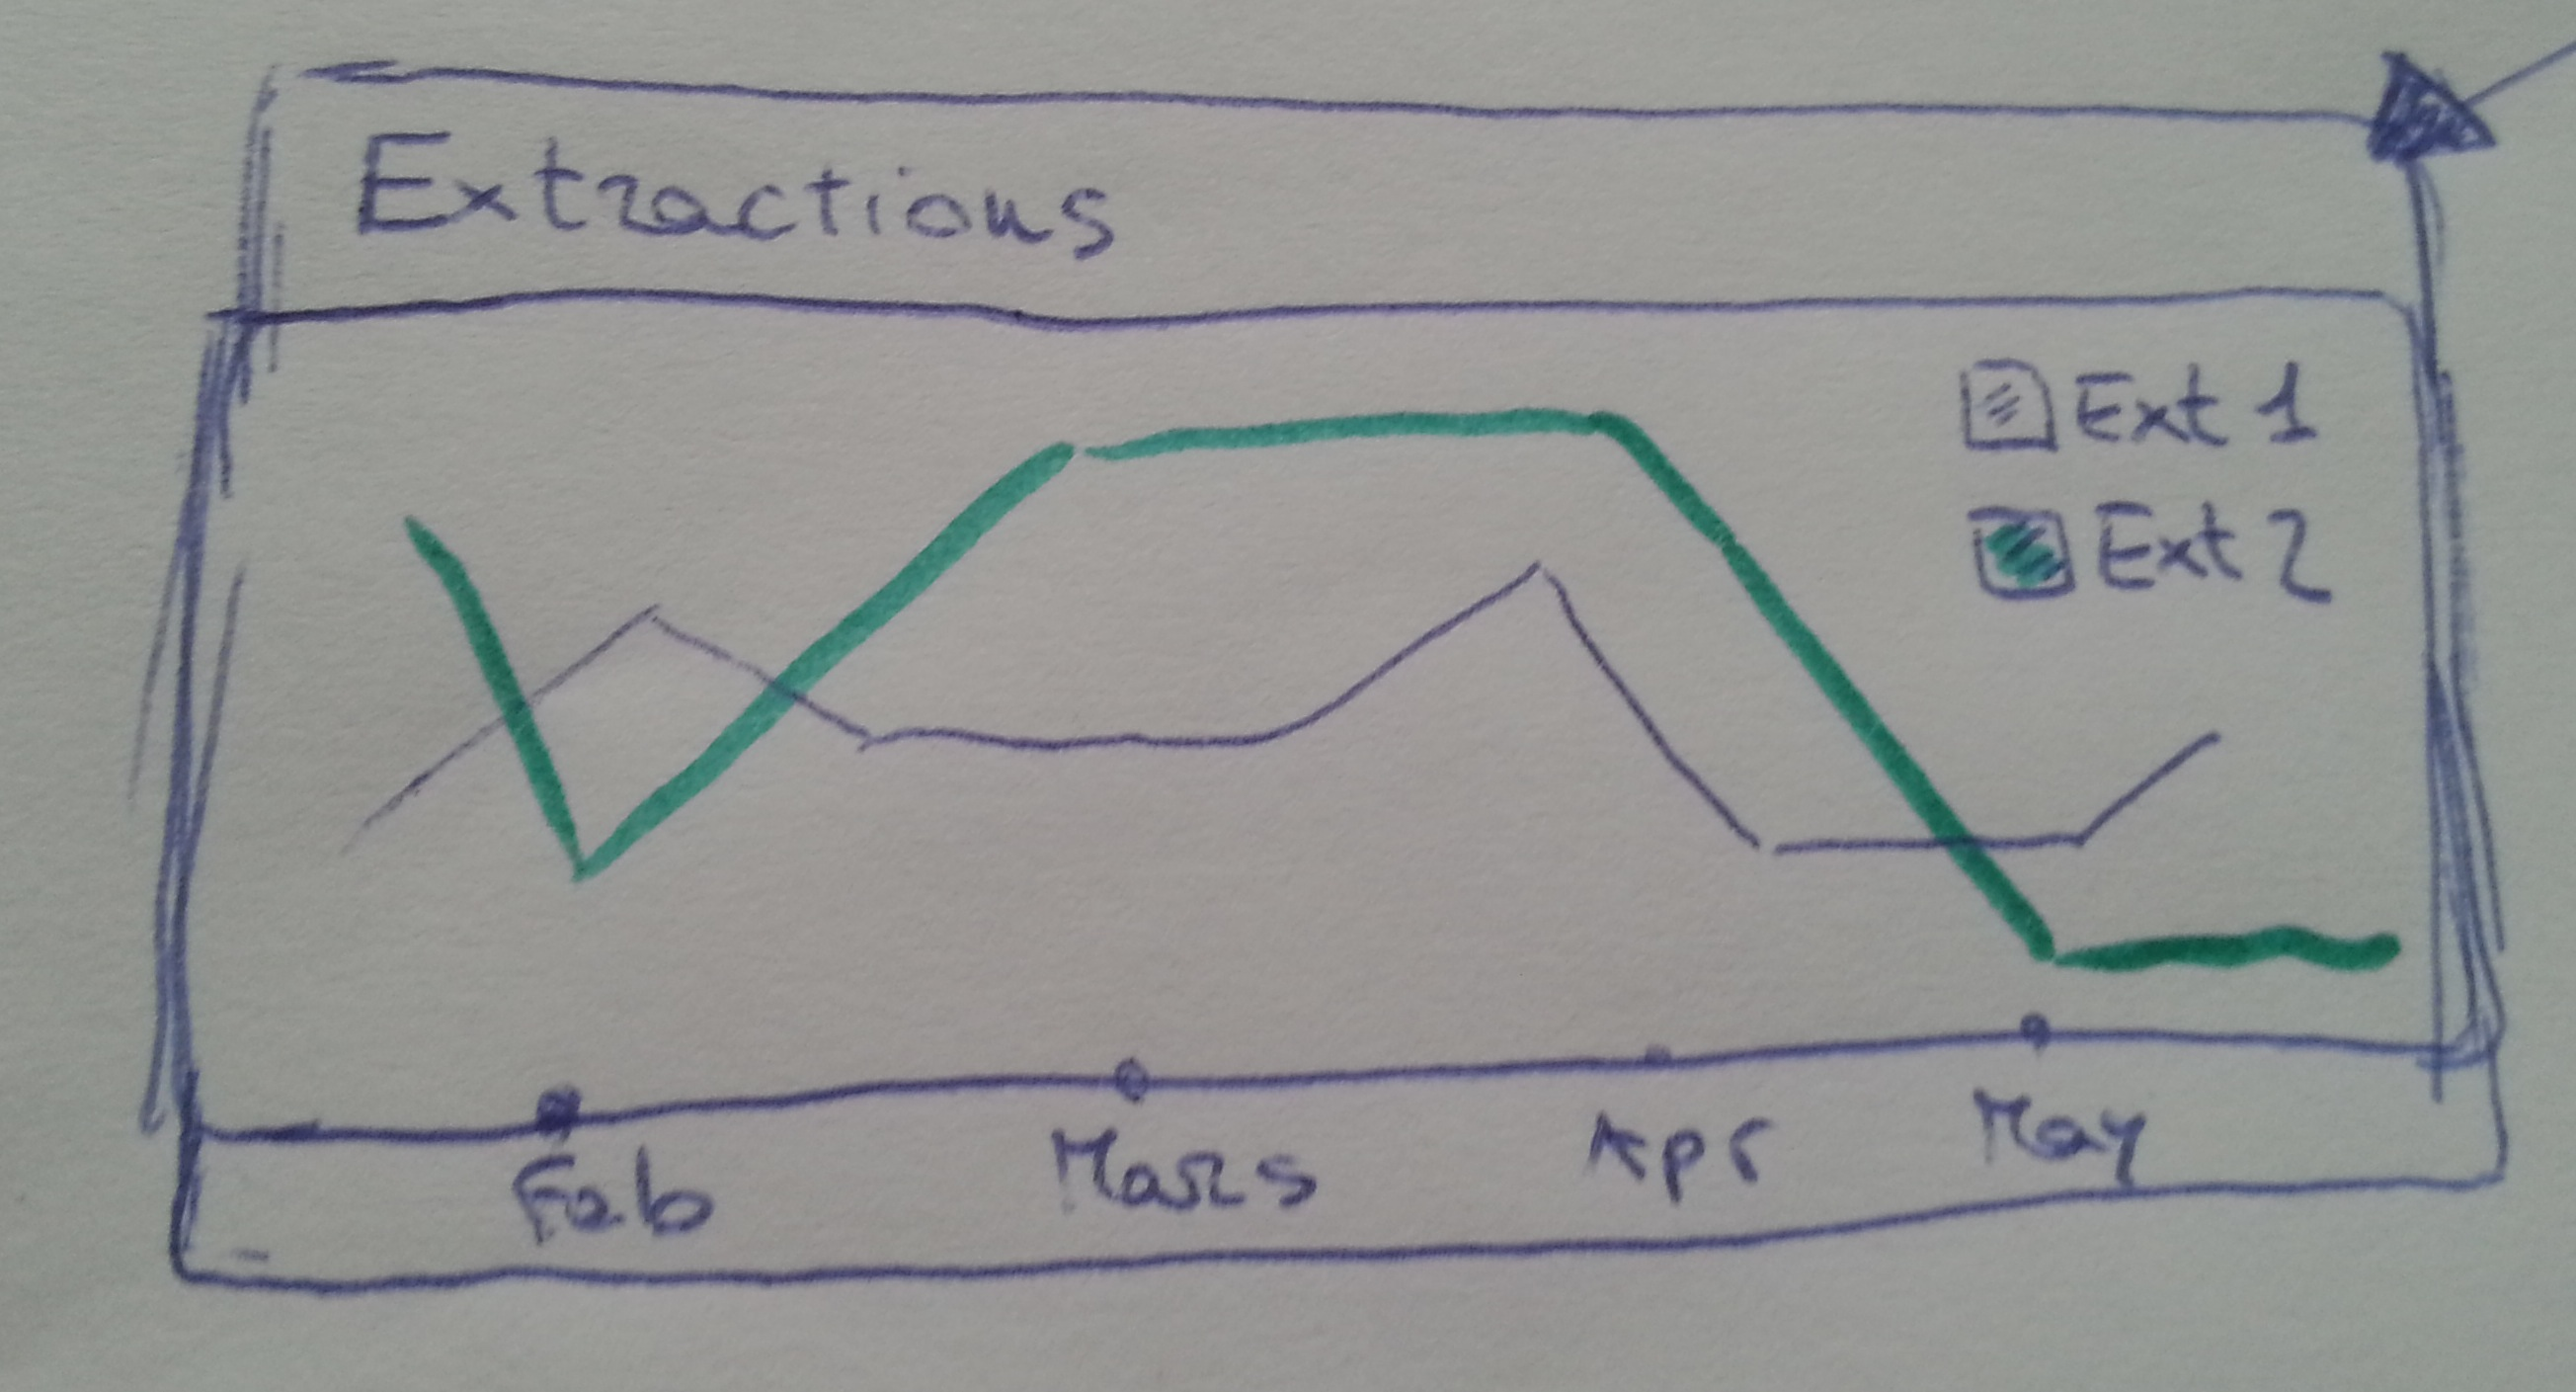
\includegraphics[width=10cm]{pics/UISketches/chart0}}
\end{figure}


\begin{figure}
\floatbox[{\capbeside\thisfloatsetup{capbesideposition={right,top},capbesidewidth=4cm}}]{figure}[\FBwidth]
{\caption{Sketches of all possible type of chart for the visualization of the NERD dashboard data.}\label{fig:test}}
{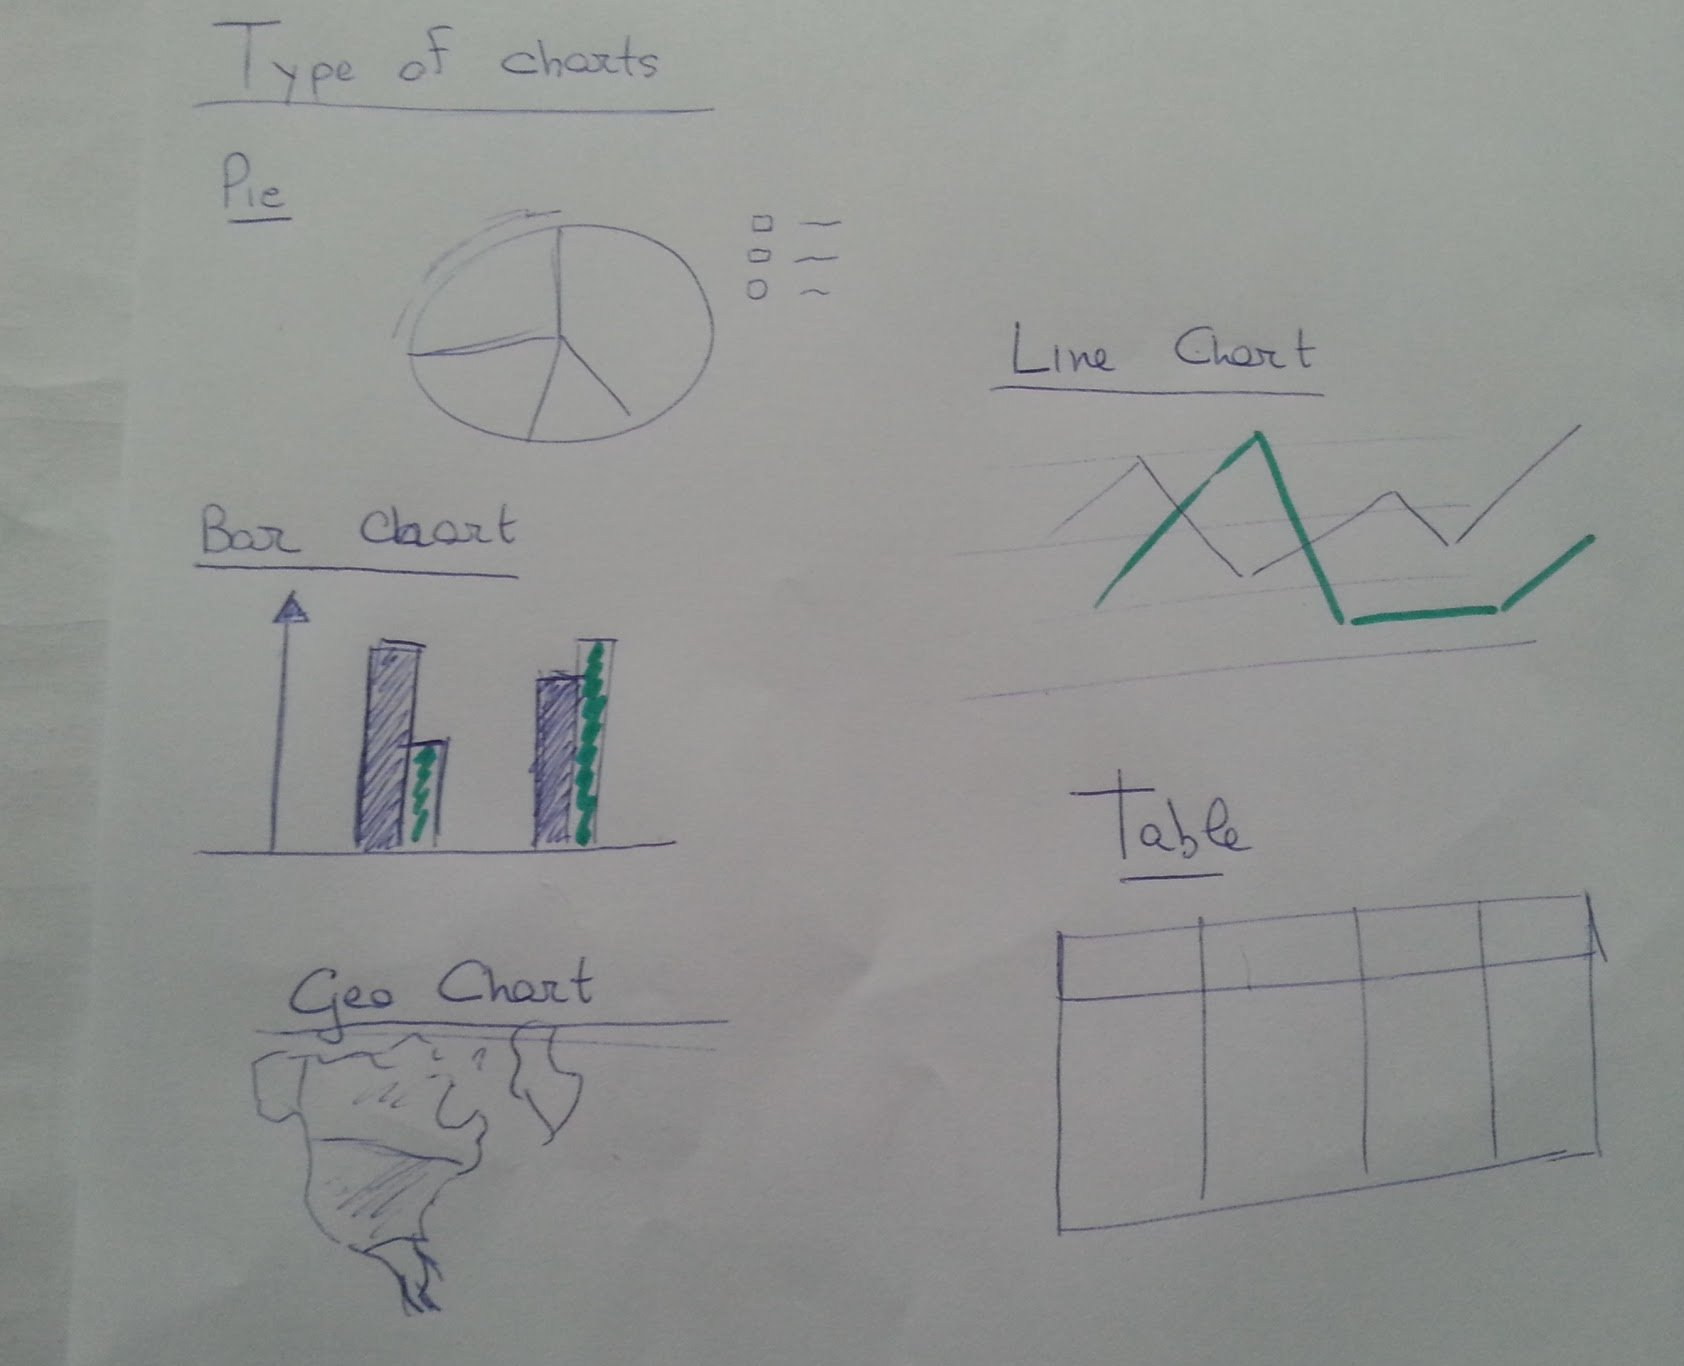
\includegraphics[width=10cm]{pics/UISketches/chart1}}
\end{figure}
\FloatBarrier
\end{document}





